% !TEX program = xelatex
\documentclass[UTF8,a4paper,10pt]{ctexart}
\usepackage[margin=2.05cm]{geometry}
\usepackage{graphicx}
\usepackage{booktabs}
\usepackage{longtable}
\usepackage{tabularx}
\usepackage{array}
\usepackage{amsmath}
\usepackage{xcolor}
\usepackage{hyperref}
\usepackage{caption}
\usepackage{float}
\usepackage[section]{placeins}
\usepackage[numbers,sort&compress]{natbib}
\graphicspath{{figures/}}
% Generated by scripts/generate_dataset_figures.py.
\newcommand{\DatasetSceneCount}{10}
\newcommand{\DatasetTiffCount}{60}
\newcommand{\DatasetUsablePatchCount}{1800}
\newcommand{\DatasetPrivacyExcludedCount}{25}
\newcommand{\DatasetFixedTrainCount}{1141}
\newcommand{\DatasetFixedValidationCount}{270}
\newcommand{\DatasetFixedTestCount}{389}
\newcommand{\DatasetTaskFileCount}{14400}
\newcommand{\DatasetRawFileCount}{1281}
\newcommand{\DatasetSourcePositionCount}{140}
\newcommand{\DatasetRgbFrameCount}{581}
\newcommand{\DatasetSwirFrameCount}{700}
\newcommand{\DatasetPoseEdgeCount}{591}
\newcommand{\DatasetOutputScale}{3.2}
\newcommand{\DatasetAcquisitionDateMin}{2025-04-29}
\newcommand{\DatasetAcquisitionDateMax}{2025-11-28}
\newcommand{\DatasetCoverageMin}{0.712}
\newcommand{\DatasetCoverageMax}{0.902}
\newcommand{\DatasetCoverageMean}{0.841}
\newcommand{\DatasetBuildSecondsMin}{48.6}
\newcommand{\DatasetBuildSecondsMax}{908.1}
\newcommand{\DatasetRedactedSceneUsablePatchCount}{131}
\newcommand{\RegHoldoutMinPx}{3.56}
\newcommand{\RegHoldoutMedianPx}{5.73}
\newcommand{\RegHoldoutMeanPx}{6.06}
\newcommand{\RegHoldoutMaxPx}{9.23}
\newcommand{\RegCornerMinPx}{1.56}
\newcommand{\RegCornerMedianPx}{3.03}
\newcommand{\RegCornerMeanPx}{5.70}
\newcommand{\RegCornerMaxPx}{27.78}
\newcommand{\RegCornerWorstScene}{C5}
\newcommand{\RegCornerRunnerUpPx}{8.60}
\newcommand{\RegCornerOutlierRatio}{3.2}
\newcommand{\RegCornerOtherMeanPx}{3.24}
\newcommand{\RegCornerGateMinPx}{25.6}
\newcommand{\RegCornerGateMaxPx}{76.3}
\newcommand{\IntraSwirMinPx}{3.19}
\newcommand{\IntraSwirMeanPx}{4.74}
\newcommand{\IntraSwirMaxPx}{6.25}
\newcommand{\IntraSwirGatePx}{8}

% Generated by scripts/build_geom_diagnostics.py; do not edit manually.
\newcommand{\GeomRgbBOnePrevMin}{0.77}
\newcommand{\GeomRgbBOnePrevMax}{1.92}
\newcommand{\GeomRgbBOneOutMin}{3.56}
\newcommand{\GeomRgbBOneOutMax}{12.97}
\newcommand{\GeomCornerPrevMin}{0.28}
\newcommand{\GeomCornerPrevMax}{1.72}
\newcommand{\GeomIntraSwirMin}{3.48}
\newcommand{\GeomIntraSwirMax}{6.25}
\newcommand{\GeomBaBeforeMin}{0.42}
\newcommand{\GeomBaBeforeMax}{2.26}
\newcommand{\GeomBaAfterMin}{0.41}
\newcommand{\GeomBaAfterMax}{0.84}
\newcommand{\GeomBaHoldoutMin}{1.06}
\newcommand{\GeomBaHoldoutMax}{2.08}
\newcommand{\GeomCovMin}{71.2}
\newcommand{\GeomCovMax}{89.2}

\newcommand{\AuditTotalTiles}{432}
\newcommand{\AuditTotalChecks}{6480}
\newcommand{\AuditJudgeablePct}{71.3}
\newcommand{\AuditRgbSwirMed}{2.37}
\newcommand{\AuditRgbSwirRmse}{3.85}
\newcommand{\AuditRgbSwirPnineFive}{7.97}
\newcommand{\AuditRgbSwirJudPct}{49.8}
\newcommand{\AuditSwirSwirMed}{0.51}
\newcommand{\AuditSwirSwirRmse}{1.73}
\newcommand{\AuditSwirSwirPnineFive}{2.84}
\newcommand{\AuditSwirSwirJudPct}{82.0}
\newcommand{\AuditRgbHiMed}{2.20}
\newcommand{\AuditRgbLoMed}{2.68}
\newcommand{\AuditSwirHiMed}{0.50}
\newcommand{\AuditSwirLoMed}{0.54}

\newcommand{\TrackCDrZsPsnr}{13.378}
\newcommand{\TrackCDrZsDe}{23.505}
\newcommand{\TrackCDrScPsnr}{14.458}
\newcommand{\TrackCDrScDe}{17.728}
\newcommand{\TrackCDrFtPsnr}{14.448}
\newcommand{\TrackCDrFtDe}{17.808}
\newcommand{\TrackCDrFtGainZs}{+1.070}
\newcommand{\TrackCDrFtGainQuad}{-2.267}

% Generated from bundled saved records; do not edit.
\newcommand{\SupportPixelCount}{88861466}
\newcommand{\QualifiedWindowCount}{5893}
\newcommand{\LpipsRectCount}{1541}
\newcommand{\FormalRunCount}{225}
\newcommand{\RandomRunCount}{45}
\newcommand{\ProtocolGain}{4.435}
\newcommand{\CalibrationAffineGain}{2.389}
\newcommand{\CalibrationQuadIncrement}{0.213}
\newcommand{\CalibrationCross}{14.113}
\newcommand{\CalibrationTarget}{16.502}
\newcommand{\CalibrationQuad}{16.715}
\newcommand{\HalfWithin}{17.432}
\newcommand{\HalfCross}{15.587}
\newcommand{\HalfDrop}{1.845}
\newcommand{\DrunetGain}{0.202}
\newcommand{\DrunetSingle}{13.619}
\newcommand{\DrunetTriple}{13.820}
\newcommand{\PixGain}{-0.020}
\newcommand{\PixSingle}{12.876}
\newcommand{\PixTriple}{12.856}
\newcommand{\TfdGain}{0.800}
\newcommand{\TfdSingle}{12.040}
\newcommand{\TfdTriple}{12.839}

\newcommand{\MsEpHundredPsnr}{25.22}
\newcommand{\MsEpHundredPsnrSd}{--}
\newcommand{\MsEpHundredPsnrPm}{25.22}
\newcommand{\MsEpHundredSsim}{0.815}
\newcommand{\MsEpHundredSsimSd}{--}
\newcommand{\MsEpHundredSsimPm}{0.815}
\newcommand{\MsEpHundredLpips}{0.068}
\newcommand{\MsEpHundredLpipsSd}{--}
\newcommand{\MsEpHundredLpipsPm}{0.068}
\newcommand{\MsEpTwoHundredPsnr}{28.81}
\newcommand{\MsEpTwoHundredPsnrSd}{--}
\newcommand{\MsEpTwoHundredPsnrPm}{28.81}
\newcommand{\MsEpTwoHundredSsim}{0.871}
\newcommand{\MsEpTwoHundredSsimSd}{--}
\newcommand{\MsEpTwoHundredSsimPm}{0.871}
\newcommand{\MsEpTwoHundredLpips}{0.033}
\newcommand{\MsEpTwoHundredLpipsSd}{--}
\newcommand{\MsEpTwoHundredLpipsPm}{0.033}
\newcommand{\ChEpHundredPsnr}{18.18}
\newcommand{\ChEpHundredPsnrSd}{--}
\newcommand{\ChEpHundredPsnrPm}{18.18}
\newcommand{\ChEpHundredSsim}{0.627}
\newcommand{\ChEpHundredSsimSd}{--}
\newcommand{\ChEpHundredSsimPm}{0.627}
\newcommand{\ChEpHundredLpips}{0.202}
\newcommand{\ChEpHundredLpipsSd}{--}
\newcommand{\ChEpHundredLpipsPm}{0.202}
\newcommand{\ChEpTwoHundredPsnr}{22.87}
\newcommand{\ChEpTwoHundredPsnrSd}{--}
\newcommand{\ChEpTwoHundredPsnrPm}{22.87}
\newcommand{\ChEpTwoHundredSsim}{0.739}
\newcommand{\ChEpTwoHundredSsimSd}{--}
\newcommand{\ChEpTwoHundredSsimPm}{0.739}
\newcommand{\ChEpTwoHundredLpips}{0.075}
\newcommand{\ChEpTwoHundredLpipsSd}{--}
\newcommand{\ChEpTwoHundredLpipsPm}{0.075}
\newcommand{\NativeEpHundredPsnr}{18.02}
\newcommand{\NativeEpHundredPsnrSd}{--}
\newcommand{\NativeEpHundredPsnrPm}{18.02}
\newcommand{\NativeEpHundredSsim}{0.551}
\newcommand{\NativeEpHundredSsimSd}{--}
\newcommand{\NativeEpHundredSsimPm}{0.551}
\newcommand{\NativeEpHundredLpips}{0.404}
\newcommand{\NativeEpHundredLpipsSd}{--}
\newcommand{\NativeEpHundredLpipsPm}{0.404}
\newcommand{\NativeEpTwoHundredPsnr}{20.72}
\newcommand{\NativeEpTwoHundredPsnrSd}{--}
\newcommand{\NativeEpTwoHundredPsnrPm}{20.72}
\newcommand{\NativeEpTwoHundredSsim}{0.577}
\newcommand{\NativeEpTwoHundredSsimSd}{--}
\newcommand{\NativeEpTwoHundredSsimPm}{0.577}
\newcommand{\NativeEpTwoHundredLpips}{0.283}
\newcommand{\NativeEpTwoHundredLpipsSd}{--}
\newcommand{\NativeEpTwoHundredLpipsPm}{0.283}
\newcommand{\MsEpFiveHundredPsnr}{30.18}
\newcommand{\MsEpFiveHundredPsnrSd}{--}
\newcommand{\MsEpFiveHundredPsnrPm}{30.18}
\newcommand{\MsEpFiveHundredSsim}{0.905}
\newcommand{\MsEpFiveHundredSsimSd}{--}
\newcommand{\MsEpFiveHundredSsimPm}{0.905}
\newcommand{\MsEpFiveHundredLpips}{0.025}
\newcommand{\MsEpFiveHundredLpipsSd}{--}
\newcommand{\MsEpFiveHundredLpipsPm}{0.025}
\newcommand{\ChEpFiveHundredPsnr}{23.25}
\newcommand{\ChEpFiveHundredPsnrSd}{0.59}
\newcommand{\ChEpFiveHundredPsnrPm}{23.25$\pm$0.59}
\newcommand{\ChEpFiveHundredSsim}{0.774}
\newcommand{\ChEpFiveHundredSsimSd}{0.004}
\newcommand{\ChEpFiveHundredSsimPm}{0.774$\pm$0.004}
\newcommand{\ChEpFiveHundredLpips}{0.079}
\newcommand{\ChEpFiveHundredLpipsSd}{0.017}
\newcommand{\ChEpFiveHundredLpipsPm}{0.079$\pm$0.017}
\newcommand{\FracTwentyFivePsnr}{--}
\newcommand{\FracTwentyFivePsnrSd}{--}
\newcommand{\FracTwentyFivePsnrPm}{--}
\newcommand{\FracTwentyFiveSsim}{--}
\newcommand{\FracTwentyFiveSsimSd}{--}
\newcommand{\FracTwentyFiveSsimPm}{--}
\newcommand{\FracTwentyFiveLpips}{--}
\newcommand{\FracTwentyFiveLpipsSd}{--}
\newcommand{\FracTwentyFiveLpipsPm}{--}
\newcommand{\FracFiftyPsnr}{--}
\newcommand{\FracFiftyPsnrSd}{--}
\newcommand{\FracFiftyPsnrPm}{--}
\newcommand{\FracFiftySsim}{--}
\newcommand{\FracFiftySsimSd}{--}
\newcommand{\FracFiftySsimPm}{--}
\newcommand{\FracFiftyLpips}{--}
\newcommand{\FracFiftyLpipsSd}{--}
\newcommand{\FracFiftyLpipsPm}{--}
\newcommand{\FracSeventyFivePsnr}{--}
\newcommand{\FracSeventyFivePsnrSd}{--}
\newcommand{\FracSeventyFivePsnrPm}{--}
\newcommand{\FracSeventyFiveSsim}{--}
\newcommand{\FracSeventyFiveSsimSd}{--}
\newcommand{\FracSeventyFiveSsimPm}{--}
\newcommand{\FracSeventyFiveLpips}{--}
\newcommand{\FracSeventyFiveLpipsSd}{--}
\newcommand{\FracSeventyFiveLpipsPm}{--}
\newcommand{\SceneFoldAPsnr}{--}
\newcommand{\SceneFoldAPsnrSd}{--}
\newcommand{\SceneFoldAPsnrPm}{--}
\newcommand{\SceneFoldASsim}{--}
\newcommand{\SceneFoldASsimSd}{--}
\newcommand{\SceneFoldASsimPm}{--}
\newcommand{\SceneFoldALpips}{--}
\newcommand{\SceneFoldALpipsSd}{--}
\newcommand{\SceneFoldALpipsPm}{--}
\newcommand{\SceneFoldBPsnr}{--}
\newcommand{\SceneFoldBPsnrSd}{--}
\newcommand{\SceneFoldBPsnrPm}{--}
\newcommand{\SceneFoldBSsim}{--}
\newcommand{\SceneFoldBSsimSd}{--}
\newcommand{\SceneFoldBSsimPm}{--}
\newcommand{\SceneFoldBLpips}{--}
\newcommand{\SceneFoldBLpipsSd}{--}
\newcommand{\SceneFoldBLpipsPm}{--}
\newcommand{\MsEpHundredSeeds}{1}
\newcommand{\ChEpHundredSeeds}{1}
\newcommand{\ChEpTwoHundredSeeds}{1}
\newcommand{\NativeDropHundred}{7.20}
\newcommand{\NativeDropTwoHundred}{8.09}
\newcommand{\ChLateSwing}{0.84}
\newcommand{\GapEpHundred}{+7.04}
\newcommand{\GapEpTwoHundred}{+5.93}
\newcommand{\MsSceneMinPsnr}{22.16}
\newcommand{\MsSceneMaxPsnr}{28.70}
\newcommand{\MsSceneMinName}{C1}
\newcommand{\ChSceneMinPsnr}{15.95}
\newcommand{\ChSceneMaxPsnr}{20.80}
\newcommand{\ChSceneMinName}{1}
\newcommand{\ScaleChenLagOne}{0.961}
\newcommand{\ScaleChenPsd}{0.037}
\newcommand{\ScaleChenBLagOne}{0.923}
\newcommand{\ScaleChenBPsd}{0.054}
\newcommand{\ScaleChenAbCorr}{0.544}
\newcommand{\ScaleChenAbPeak}{0.599}
\newcommand{\ScaleChenAbRatio}{91}
\newcommand{\ScaleChenPeakWithinOnePx}{69.3}
\newcommand{\ScaleChenPeakWeakPct}{12.2}
\newcommand{\ScaleChenPeakWithinOnePxStrong}{76.1}
\newcommand{\ScaleChenRgbChanCorr}{0.681}
\newcommand{\ScaleChenRgbSat}{2.8/1.8/2.2}
\newcommand{\ScaleMsLagOne}{0.963}
\newcommand{\ScaleMsPsd}{0.035}
\newcommand{\ScaleMsBLagOne}{0.936}
\newcommand{\ScaleMsBPsd}{0.047}
\newcommand{\ScaleMsAbCorr}{0.499}
\newcommand{\ScaleMsAbPeak}{0.548}
\newcommand{\ScaleMsAbRatio}{91}
\newcommand{\ScaleMsPeakWithinOnePx}{68.0}
\newcommand{\ScaleMsPeakWeakPct}{16.9}
\newcommand{\ScaleMsPeakWithinOnePxStrong}{76.6}
\newcommand{\ScaleMsRgbChanCorr}{0.718}
\newcommand{\ScaleMsRgbSat}{8.8/7.5/8.8}
\newcommand{\ScaleNativeLagOne}{0.992}
\newcommand{\ScaleNativePsd}{0.018}
\newcommand{\ScaleNativeBLagOne}{0.974}
\newcommand{\ScaleNativeBPsd}{0.031}
\newcommand{\ScaleNativeAbCorr}{0.585}
\newcommand{\ScaleNativeAbPeak}{0.654}
\newcommand{\ScaleNativeAbRatio}{89}
\newcommand{\ScaleNativePeakWithinOnePx}{25.7}
\newcommand{\ScaleNativePeakWeakPct}{9.9}
\newcommand{\ScaleNativePeakWithinOnePxStrong}{28.2}
\newcommand{\ScaleNativeRgbChanCorr}{0.750}
\newcommand{\ScaleNativeRgbSat}{5.6/3.8/7.5}
\newcommand{\ScaleNativePeakWithinFourPx}{71.4}
\newcommand{\BandBOneMeanMin}{120}
\newcommand{\BandBOneMeanMax}{201}
\newcommand{\BandBOneSat}{4.96}
\newcommand{\BandBOneSatMax}{12.5}
\newcommand{\BandBOneCorrMin}{0.690}
\newcommand{\BandBOneCorrMax}{0.993}
\newcommand{\BandBOneLumaMin}{-0.10}
\newcommand{\BandBOneLumaMax}{+0.84}
\newcommand{\BandBTwoMeanMin}{111}
\newcommand{\BandBTwoMeanMax}{175}
\newcommand{\BandBTwoSat}{1.62}
\newcommand{\BandBTwoSatMax}{6.5}
\newcommand{\BandBTwoCorrMin}{0.600}
\newcommand{\BandBTwoCorrMax}{0.994}
\newcommand{\BandBTwoLumaMin}{-0.17}
\newcommand{\BandBTwoLumaMax}{+0.83}
\newcommand{\BandBThreeMeanMin}{83}
\newcommand{\BandBThreeMeanMax}{142}
\newcommand{\BandBThreeSat}{0.12}
\newcommand{\BandBThreeSatMax}{1.0}
\newcommand{\BandBThreeCorrMin}{0.600}
\newcommand{\BandBThreeCorrMax}{0.997}
\newcommand{\BandBThreeLumaMin}{+0.23}
\newcommand{\BandBThreeLumaMax}{+0.79}
\newcommand{\BandBFourMeanMin}{101}
\newcommand{\BandBFourMeanMax}{154}
\newcommand{\BandBFourSat}{0.39}
\newcommand{\BandBFourSatMax}{1.5}
\newcommand{\BandBFourCorrMin}{0.677}
\newcommand{\BandBFourCorrMax}{0.994}
\newcommand{\BandBFourLumaMin}{-0.18}
\newcommand{\BandBFourLumaMax}{+0.83}
\newcommand{\BandBFiveMeanMin}{86}
\newcommand{\BandBFiveMeanMax}{138}
\newcommand{\BandBFiveSat}{0.10}
\newcommand{\BandBFiveSatMax}{1.0}
\newcommand{\BandBFiveCorrMin}{0.686}
\newcommand{\BandBFiveCorrMax}{0.997}
\newcommand{\BandBFiveLumaMin}{+0.14}
\newcommand{\BandBFiveLumaMax}{+0.79}
\newcommand{\CorrWithinMin}{0.898}
\newcommand{\CorrWithinMedian}{0.987}
\newcommand{\CorrWithinMax}{0.997}
\newcommand{\CorrCrossMin}{0.600}
\newcommand{\CorrCrossMedian}{0.869}
\newcommand{\CorrCrossMax}{0.975}
\newcommand{\BandBOneSatTopName}{C1}
\newcommand{\BandBOneSatTop}{12.5}
\newcommand{\BandBOneSatSecondName}{C5}
\newcommand{\BandBOneSatSecond}{10.6}
\newcommand{\RgbSatMaxName}{C8}
\newcommand{\RgbSatMax}{34.6}
\newcommand{\RgbSatSecond}{23.4}
\newcommand{\RgbZeroMaxName}{C9}
\newcommand{\RgbZeroMaxChannel}{蓝}
\newcommand{\RgbZeroMax}{25.9}
\newcommand{\SceneAlignMinName}{C5}
\newcommand{\SceneAlignMin}{51.6}
\newcommand{\SceneAlignMaxName}{C3}
\newcommand{\SceneAlignMax}{100.0}
\newcommand{\SceneCorrMin}{0.26}
\newcommand{\SceneCorrMax}{0.87}
\newcommand{\SceneWeakMaxName}{C7}
\newcommand{\SceneWeakMax}{31.7}
\newcommand{\SceneWeakSecondName}{C9}
\newcommand{\SceneWeakSecond}{30.0}
\newcommand{\ScaleMsWeakStd}{22.9}
\newcommand{\ScaleMsStrongStd}{27.7}
\newcommand{\SeedsDone}{0}
\newcommand{\BandDone}{0}
\newcommand{\SceneDone}{0}
\newcommand{\BudgetDone}{0}
\newcommand{\QualPsnrMin}{19.33}
\newcommand{\QualPsnrMax}{26.88}

\hypersetup{colorlinks=true,linkcolor=black,citecolor=black,urlcolor=blue}
\setlength{\parindent}{2em}
\setlength{\parskip}{0.25em}
\setlength{\emergencystretch}{2em}
\captionsetup{font=small,labelfont=bf}
\renewcommand{\arraystretch}{1.15}
\renewcommand{\thetable}{S\arabic{table}}
\renewcommand{\thefigure}{S\arabic{figure}}
\newcommand{\dE}{\ensuremath{\Delta E_{00}}}

\title{\textbf{补充材料（Supplementary Information）}\\[0.35em]\large M-SWIR-RGB：面向跨光谱图像生成的场景级RGB与五波段短波红外配对数据集}
\author{杜虎$^{1,2,*}$，刘晓$^{2,3,\dagger}$，杜丽丽$^{2,3}$，崔虎$^{2}$\\[0.3em]
\small $^{1}$中国科学技术大学，合肥 230026，中国\\
\small $^{2}$中国科学院合肥物质科学研究院，合肥 230031，中国\\
\small $^{3}$中国科学院安徽光学精密机械研究所光学定标与表征重点实验室，合肥 230031，中国}
\date{}

\begin{document}\maketitle

本补充材料提供M-SWIR-RGB数据描述符\cite{du2026mswirrgb_data}配套的逐地点质量诊断与波段两两相关矩阵、轨道A更新预算与消融明细、轨道B地点隔离五折划分与45种固定输入全表、评价支持度统计以及验证轨迹曲线，与英文版补充材料严格一一对应。

\section*{补充节 1：逐地点质量裁剪、窗口对齐与波段两两相关性}

\begin{table}[htbp]\centering\footnotesize\setlength{\tabcolsep}{3pt}
\caption{逐地点的像素裁剪比例与模态间灰度对齐统计（4:1窗口）。}\label{tab:s-quality-scene-zh}
\vspace{1pt}{\footnotesize\noindent B1取255比例按成图几何有效区域内每隔7像素抽样统计；其余各列按4:1窗口计，RGB取255与取0两列依次为R/G/B三通道，零位移相关取窗口中位数。$^{*}$末列分母为该地点峰值相关$r_{\mathrm{p}}\geq0.2$的可判定窗口。\par}
\begin{tabular}{@{}lrrrrrrrr@{}}
\toprule
场景 & 窗口 & B1取255/\% & RGB均值 & RGB取255/\% & RGB取0/\% & 零位移相关 & 不可判定/\% & 位移$\le$1像素$^{*}$/\%\\
\midrule
C1 & 819 & 12.5 & 156 & 14.9/3.4/12.9 & 0.2/1.3/2.2 & 0.47 & 22.3 & 73.9 \\
C2 & 595 & 0.1 & 60 & 4.4/0.2/0.2 & 7.6/1.9/4.6 & 0.87 & 0.0 & 91.9 \\
C3 & 130 & 0.5 & 57 & 1.1/0.6/0.9 & 0.8/0.3/4.6 & 0.64 & 9.2 & 100.0 \\
C4 & 110 & 2.4 & 82 & 0.9/0.0/0.0 & 0.1/0.0/1.0 & 0.70 & 14.5 & 87.2 \\
C5 & 280 & 10.6 & 93 & 3.9/0.4/3.8 & 0.4/0.1/2.6 & 0.59 & 1.8 & 51.6 \\
C6 & 165 & 5.4 & 130 & 2.3/2.3/23.4 & 0.6/0.0/0.1 & 0.71 & 1.2 & 80.4 \\
C7 & 328 & 8.0 & 130 & 6.3/6.2/12.8 & 0.1/0.0/0.8 & 0.31 & 31.7 & 81.7 \\
C8 & 672 & 0.0 & 144 & 33.7/34.6/34.3 & 0.0/0.0/0.0 & 0.40 & 23.8 & 69.1 \\
C9 & 377 & 0.0 & 55 & 9.6/9.0/7.8 & 0.3/0.1/25.9 & 0.26 & 30.0 & 65.5 \\
C10 & 76 & 4.2 & 90 & 6.3/8.4/10.3 & 7.6/1.6/2.0 & 0.62 & 7.9 & 85.7 \\
\bottomrule
\end{tabular}

\end{table}

\begin{table}[htbp]\centering\small
\caption{五个SWIR波段两两Pearson相关系数在十个地点上的分布。}\label{tab:s-quality-corr-zh}
\vspace{1pt}{\footnotesize\noindent 在每个地点成图几何有效区域内每隔7个有效像素抽样计算Pearson系数，汇总十地点的最小值、中位数与最大值。\par}
\begin{tabular}{@{}lrrr@{}}
\toprule
波段对 & 十场景最小 & 中位数 & 最大\\
\midrule
B1--B2 & 0.953 & 0.987 & 0.993 \\
B1--B3 & 0.690 & 0.855 & 0.945 \\
B1--B4 & 0.898 & 0.975 & 0.990 \\
B1--B5 & 0.777 & 0.888 & 0.946 \\
B2--B3 & 0.600 & 0.822 & 0.940 \\
B2--B4 & 0.944 & 0.987 & 0.994 \\
B2--B5 & 0.686 & 0.870 & 0.935 \\
B3--B4 & 0.677 & 0.868 & 0.972 \\
B3--B5 & 0.967 & 0.989 & 0.997 \\
B4--B5 & 0.765 & 0.900 & 0.975 \\
\bottomrule
\end{tabular}

\end{table}

\clearpage
\section*{补充节 2：轨道A预算、逐场景种子结果、三架构兼容与消融明细}

\begin{table}[htbp]\centering\small
\caption{轨道A窗口级基准的数据规模与参数更新预算。}\label{tab:s-bench-protocol-zh}
\vspace{1pt}{\footnotesize\noindent 除“窗口尺度”一行外均使用4:1窗口；对照归档使用现成图块。更新次数为每轮实际批次数与epoch数之积。\par}
\begin{tabular}{@{}llrrl@{}}\toprule
实验 & 训练集 & 训练窗口 & 测试窗口 & 更新次数\\\midrule
同配置对照 & M-SWIR-RGB & 2{,}842 & 710 & 71{,}000 / 142{,}000\\
同配置对照 & 七场景对照归档\cite{chen2026thesis} & 2{,}972 & 743 & 74{,}300 / 148{,}600\\
输入波段消融 & M-SWIR-RGB，15种输入 & 2{,}842 & 710 & 71{,}000\\
训练数据量 & M-SWIR-RGB 25\%/50\%/75\% & 710/1{,}422/2{,}132 & 710 & 70{,}800/71{,}000/69{,}290\\
窗口尺度 & M-SWIR-RGB 1:1窗口 & 3{,}109 & 777 & 77{,}700 / 155{,}400\\
场景划分A/B & C1--C5 / C6--C10 & 1{,}558/1{,}284 & 1{,}618/1{,}934 & 70{,}020 / 70{,}620\\\bottomrule
\end{tabular}\end{table}

\begin{table}[htbp]\centering\small
\caption{M-SWIR-RGB逐场景的同配置窗口级结果（100 epoch）。}\label{tab:s-bench-scene-seeds-zh}
\vspace{1pt}{\footnotesize\noindent 测试窗口算术平均；PSNR列给出三次独立训练的均值$\pm$样本标准差。\par}
\begin{tabular}{@{}lrrrr@{}}
\toprule
场景 & 测试窗口 & PSNR/dB$\uparrow$ & SSIM$\uparrow$ & LPIPS$\downarrow$\\
\midrule
C1 & 164 & 22.16 & 0.800 & 0.060 \\
C2 & 116 & 27.61 & 0.850 & 0.034 \\
C3 & 18 & 25.43 & 0.827 & 0.079 \\
C4 & 18 & 24.35 & 0.630 & 0.217 \\
C5 & 60 & 23.54 & 0.793 & 0.058 \\
C6 & 37 & 25.04 & 0.811 & 0.070 \\
C7 & 62 & 23.85 & 0.782 & 0.085 \\
C8 & 140 & 26.64 & 0.850 & 0.075 \\
C9 & 79 & 28.70 & 0.843 & 0.076 \\
C10 & 16 & 22.43 & 0.694 & 0.091 \\
\midrule
十个场景合并 & 710 & 25.22 & 0.815 & 0.068 \\
\bottomrule
\end{tabular}

\end{table}

\begin{table}[htbp]\centering\small
\caption{同4:1数据与划分下的三类生成架构对比（200 epoch，256整块输入）。}\label{tab:s-three-model-zh}
\vspace{1pt}{\footnotesize\noindent 固定训练种子11，批大小为唯一变量。\par}
\begin{tabular}{@{}llrrr@{}}
\toprule
模型 & batch & PSNR/dB & SSIM & LPIPS-Alex\\
\midrule
pix2pix & 1 & 14.836 & 0.493 & 0.365\\
pix2pix & 4 & 25.106 & 0.769 & 0.120\\
TFD-GAN & 1 & 27.220 & 0.834 & 0.044\\
TFD-GAN & 4 & 29.054 & 0.875 & 0.033\\
DRUNet & 1 & 36.453 & 0.962 & 0.017\\
DRUNet & 4 & 36.438 & 0.961 & 0.018\\
\bottomrule
\end{tabular}

\end{table}

\begin{table}[htbp]\centering\small
\caption{轨道A输入波段消融（100 epoch，4:1随机窗口划分）。}\label{tab:s-bench-band-zh}
\vspace{1pt}{\footnotesize\noindent 单波段复制为三通道，三波段按波段号升序堆叠。$\Delta$PSNR为相对B123三次平均的逐窗口差值均值，括号内为按场景整群bootstrap的95\%置信区间。\par}
\begin{tabular}{@{}lrrrr@{}}
\toprule
输入 & PSNR/dB$\uparrow$ & SSIM$\uparrow$ & LPIPS$\downarrow$ & $\Delta$PSNR 及 95\% 置信区间\\
\midrule
B1 & -- & -- & -- & -- \\
B2 & -- & -- & -- & -- \\
B3 & -- & -- & -- & -- \\
B4 & -- & -- & -- & -- \\
B5 & -- & -- & -- & -- \\
B123（参照，1 次训练） & 25.22 & 0.815 & 0.068 & 参照 \\
B124 & -- & -- & -- & -- \\
B125 & -- & -- & -- & -- \\
B134 & -- & -- & -- & -- \\
B135 & -- & -- & -- & -- \\
B145 & -- & -- & -- & -- \\
B234 & -- & -- & -- & -- \\
B235 & -- & -- & -- & -- \\
B245 & -- & -- & -- & -- \\
B345 & -- & -- & -- & -- \\
\bottomrule
\end{tabular}

\end{table}

\begin{table}[htbp]\centering\small
\caption{匹配更新预算下的训练数据量对照（4:1窗口，固定710个测试窗口）。}\label{tab:s-bench-budget-zh}
\vspace{1pt}{\footnotesize\noindent 各子集按场景分层抽取，更新次数对齐69{,}290--71{,}000；100\%一行为3次训练均值$\pm$标准差。\par}
\begin{tabular}{@{}rrlrrr@{}}
\toprule
训练集 & 训练窗口 & 更新次数 & PSNR/dB$\uparrow$ & SSIM$\uparrow$ & LPIPS$\downarrow$\\
\midrule
25\% & 710 & 70{,}800 & 24.15 & 0.794 & 0.085 \\
50\% & 1422 & 71{,}000 & 24.68 & 0.806 & 0.071 \\
75\% & 2132 & 69{,}290 & 24.06 & 0.803 & 0.096 \\
100\% & 2842 & 71{,}000 & 24.46$\pm$1.12 & 0.807$\pm$0.011 & 0.089$\pm$0.029 \\
\bottomrule
\end{tabular}

\end{table}

\begin{figure}[htbp]\centering
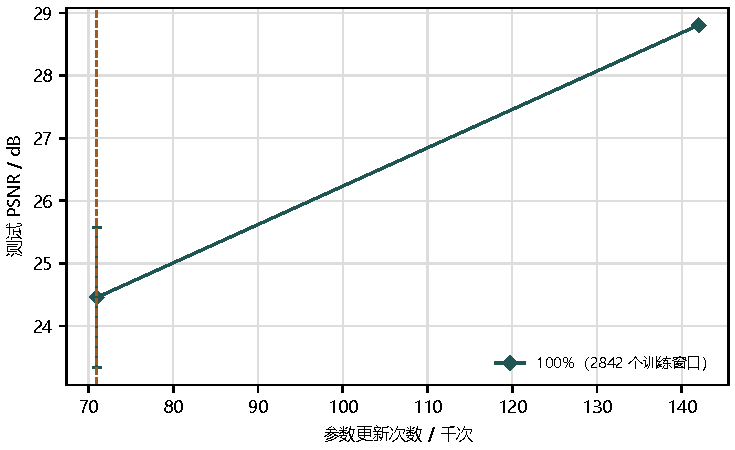
\includegraphics[width=.66\textwidth]{figures/zh/results_20261124/budget_curve_zh.pdf}
\caption{匹配更新预算下的训练数据量对比（4:1窗口，虚线标记全量100 epoch预算71{,}000次更新）。\label{fig:s-budget-curve-zh}}
\end{figure}

\begin{table}[htbp]\centering\small
\caption{逐场景在4:1随机窗口划分与两折留出场景下的PSNR对照（dB）。}\label{tab:s-bench-per-scene-zh}
\vspace{1pt}{\footnotesize\noindent 随机窗口为3次训练均值；留出场景为该场景不参与训练时的测试表现；差值为留出减随机。\par}
\begin{tabular}{@{}lrrr@{}}
\toprule
场景 & 随机窗口划分 & 留出场景 & 差值\\
\midrule
C1 & 21.71 & 5.13 & -16.57 \\
C2 & 26.37 & 9.61 & -16.75 \\
C3 & 24.85 & 11.44 & -13.40 \\
C4 & 23.30 & 10.64 & -12.65 \\
C5 & 23.26 & 9.20 & -14.06 \\
C6 & 24.44 & 9.36 & -15.08 \\
C7 & 22.91 & 7.87 & -15.03 \\
C8 & 25.74 & 8.08 & -17.66 \\
C9 & 27.82 & 5.67 & -22.15 \\
C10 & 22.28 & 8.83 & -13.45 \\
\midrule
十场景等权 & 24.27 & 8.58 & -15.68 \\
\bottomrule
\end{tabular}

\end{table}

\begin{figure}[tbp]\centering
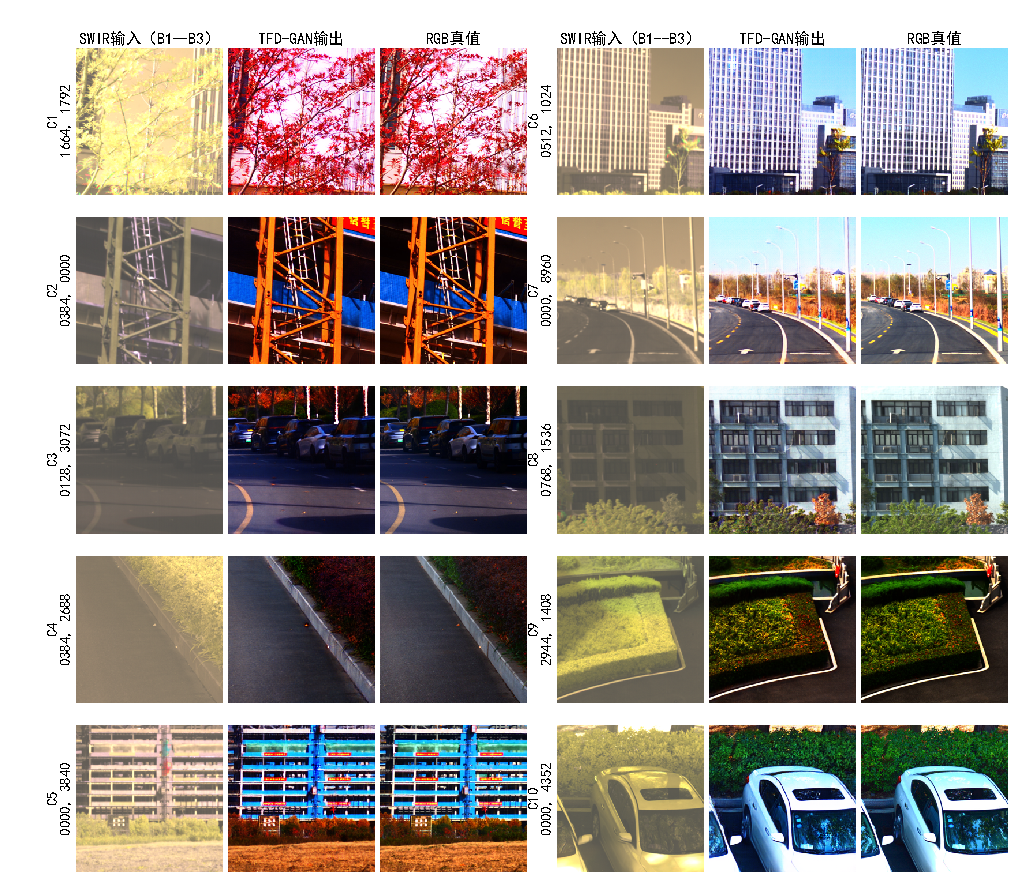
\includegraphics[width=.96\textwidth,height=.74\textheight,keepaspectratio]{figures/zh/results_20261124/qualitative_zh.pdf}
\caption{轨道A（4:1同地点随机窗口划分）下十个场景的SWIR输入、TFD-GAN输出与RGB真值示例（200 epoch，PSNR \QualPsnrMin--\QualPsnrMax\,dB）。\label{fig:s-qualitative-zh}}
\end{figure}

\clearpage
\section*{补充节 3：轨道B五折划分、45种固定输入全表、评价支持度与验证轨迹}

\begin{table}[htbp]\centering\small
\caption{地点隔离的五折交叉验证地点划分方案。}\label{tab:s-protocol-zh}
\begin{tabular}{@{}clll@{}}\toprule
折 & 训练地点（6个） & 验证地点（2个） & 测试地点（2个）\\\midrule
1 & C3,C4,C5,C6,C7,C10 & C2,C9 & C1,C8\\
2 & C1,C3,C4,C6,C7,C8 & C5,C10 & C2,C9\\
3 & C1,C2,C4,C7,C8,C9 & C3,C6 & C5,C10\\
4 & C1,C2,C5,C8,C9,C10 & C4,C7 & C3,C6\\
5 & C2,C3,C5,C6,C9,C10 & C1,C8 & C4,C7\\\bottomrule
\end{tabular}\end{table}

\begin{figure}[htbp]\centering
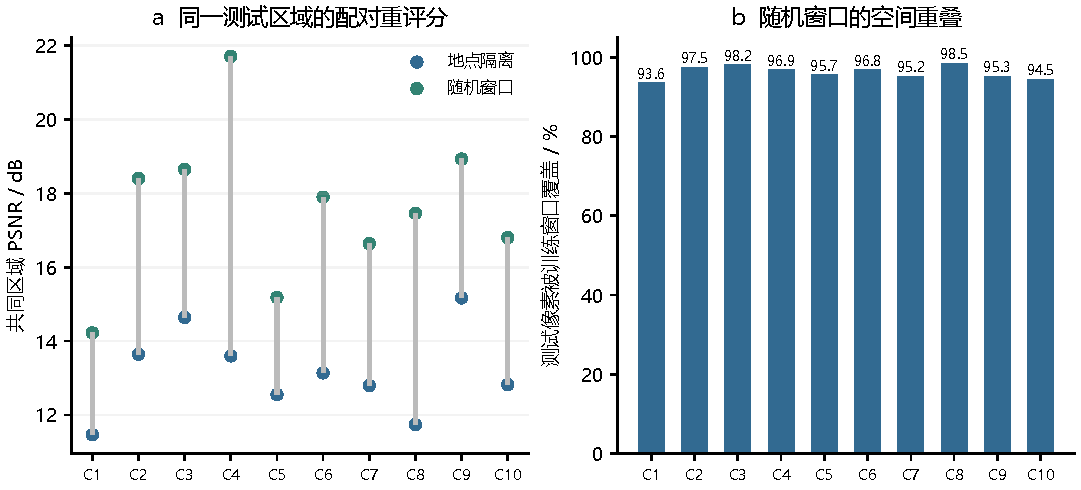
\includegraphics[width=\textwidth,height=.44\textheight,keepaspectratio]{figures/zh/results_20261109/protocol_sensitivity.pdf}
\caption{完全相同$256\times256$步长128窗口上的协议敏感性对照（pix2pix，45次随机划分与地点隔离配对重评分；平均偏高+\ProtocolGain\,dB）。\label{fig:s-protocol-sensitivity-zh}}
\end{figure}

\begin{table}[htbp]\centering\small
\caption{各折验证集选择的单波段与三波段输入。}\label{tab:s-choices-zh}
\begin{tabular}{@{}ccccccc@{}}
\toprule
折 & DRUNet单 & DRUNet三 & pix2pix单 & pix2pix三 & TFD单 & TFD三\\
\midrule
1 & S3 & T234 & S1 & T135 & S3 & T134\\
2 & S3 & T135 & S2 & T125 & S1 & T125\\
3 & S3 & T134 & S4 & T145 & S3 & T124\\
4 & S3 & T245 & S1 & T124 & S1 & T234\\
5 & S1 & T125 & S4 & T145 & S2 & T134\\
\bottomrule
\end{tabular}

\end{table}

\begingroup\small
\begin{longtable}{@{}llrrrrr@{}}
\caption{全部45种固定输入条件的十地点均值。PSNR单位为dB。}\label{tab:all-inputs-zh}\\
\toprule 模型 & 输入 & PSNR↑ & SSIM↑ & LPIPS↓ & \dE{}↓ & MAE↓\\\midrule
\endfirsthead
\multicolumn{7}{r}{\small 续表~\thetable}\\
\toprule 模型 & 输入 & PSNR↑ & SSIM↑ & LPIPS↓ & \dE{}↓ & MAE↓\\\midrule
\endhead
\midrule\multicolumn{7}{r}{续下页}\\\endfoot\bottomrule\endlastfoot
DRUNet & S1 & 13.610 & 0.578 & 0.667 & 22.102 & 0.162\\
DRUNet & S2 & 13.289 & 0.553 & 0.694 & 24.224 & 0.173\\
DRUNet & S3 & 13.629 & 0.570 & 0.688 & 22.531 & 0.164\\
DRUNet & S4 & 13.369 & 0.566 & 0.698 & 23.882 & 0.169\\
DRUNet & S5 & 13.566 & 0.568 & 0.689 & 22.569 & 0.166\\
DRUNet & T123 & 13.365 & 0.543 & 0.582 & 21.934 & 0.167\\
DRUNet & T124 & 13.347 & 0.561 & 0.621 & 23.391 & 0.163\\
DRUNet & T125 & 13.694 & 0.550 & 0.540 & 20.675 & 0.164\\
DRUNet & T134 & 13.880 & 0.554 & 0.539 & 20.249 & 0.158\\
DRUNet & T135 & 13.595 & 0.567 & 0.529 & 20.843 & 0.161\\
DRUNet & T145 & 13.588 & 0.555 & 0.590 & 21.961 & 0.164\\
DRUNet & T234 & 13.745 & 0.560 & 0.556 & 20.593 & 0.159\\
DRUNet & T235 & 13.688 & 0.545 & 0.555 & 20.952 & 0.165\\
DRUNet & T245 & 14.058 & 0.550 & 0.524 & 20.233 & 0.161\\
DRUNet & T345 & 13.519 & 0.548 & 0.579 & 21.159 & 0.166\\
pix2pix & S1 & 13.240 & 0.470 & 0.608 & 23.662 & 0.165\\
pix2pix & S2 & 12.816 & 0.471 & 0.595 & 24.733 & 0.174\\
pix2pix & S3 & 12.819 & 0.461 & 0.619 & 25.443 & 0.178\\
pix2pix & S4 & 12.663 & 0.476 & 0.594 & 24.316 & 0.178\\
pix2pix & S5 & 12.751 & 0.437 & 0.640 & 25.956 & 0.176\\
pix2pix & T123 & 12.840 & 0.452 & 0.581 & 22.546 & 0.179\\
pix2pix & T124 & 13.118 & 0.452 & 0.580 & 23.066 & 0.168\\
pix2pix & T125 & 12.929 & 0.450 & 0.576 & 23.214 & 0.176\\
pix2pix & T134 & 13.054 & 0.464 & 0.571 & 21.609 & 0.171\\
pix2pix & T135 & 13.141 & 0.436 & 0.593 & 22.687 & 0.170\\
pix2pix & T145 & 12.965 & 0.438 & 0.587 & 22.812 & 0.172\\
pix2pix & T234 & 12.929 & 0.419 & 0.656 & 22.587 & 0.175\\
pix2pix & T235 & 12.838 & 0.438 & 0.575 & 22.976 & 0.174\\
pix2pix & T245 & 12.901 & 0.394 & 0.599 & 21.918 & 0.174\\
pix2pix & T345 & 12.959 & 0.425 & 0.587 & 22.136 & 0.170\\
TFD-GAN & S1 & 11.843 & 0.417 & 0.583 & 25.956 & 0.206\\
TFD-GAN & S2 & 11.997 & 0.423 & 0.591 & 26.899 & 0.199\\
TFD-GAN & S3 & 12.376 & 0.416 & 0.562 & 26.864 & 0.189\\
TFD-GAN & S4 & 12.148 & 0.427 & 0.571 & 25.236 & 0.192\\
TFD-GAN & S5 & 12.569 & 0.421 & 0.569 & 25.896 & 0.184\\
TFD-GAN & T123 & 12.602 & 0.444 & 0.532 & 24.226 & 0.180\\
TFD-GAN & T124 & 12.887 & 0.438 & 0.530 & 23.183 & 0.173\\
TFD-GAN & T125 & 12.555 & 0.423 & 0.543 & 24.622 & 0.185\\
TFD-GAN & T134 & 12.879 & 0.448 & 0.531 & 23.084 & 0.176\\
TFD-GAN & T135 & 12.700 & 0.426 & 0.517 & 24.192 & 0.183\\
TFD-GAN & T145 & 12.760 & 0.407 & 0.564 & 24.469 & 0.182\\
TFD-GAN & T234 & 12.594 & 0.395 & 0.558 & 23.414 & 0.186\\
TFD-GAN & T235 & 12.420 & 0.407 & 0.564 & 24.755 & 0.190\\
TFD-GAN & T245 & 12.339 & 0.424 & 0.529 & 25.447 & 0.190\\
TFD-GAN & T345 & 12.576 & 0.411 & 0.560 & 24.417 & 0.186\\
\end{longtable}

\endgroup

\begin{table}[htbp]\centering\footnotesize
\caption{地点隔离主基准的逐地点评价支持（LPIPS去重覆盖比例以共同有效像素为分母）。}\label{tab:s-support-zh}
% Generated by make_support_statistics_20261015.py; counts use saved support.
\begin{tabularx}{\textwidth}{@{}>{\centering\arraybackslash}X>{\centering\arraybackslash}X>{\centering\arraybackslash}X>{\centering\arraybackslash}X>{\centering\arraybackslash}X>{\centering\arraybackslash}X>{\centering\arraybackslash}X>{\centering\arraybackslash}X@{}}
\toprule
地点 & \shortstack{公共支持\\百万像素} & \shortstack{占画布\\(\%)} & \shortstack{SSIM 中心\\百万个} & 窗口 & \shortstack{LPIPS\\矩形数} & \shortstack{去重覆盖\\百万像素} & \shortstack{覆盖/公共\\(\%)} \\
\midrule
C1 & 10.653 & 48.97 & 5.153 & 754 & 10 & 0.164 & 1.54 \\
C2 & 13.189 & 77.49 & 7.243 & 936 & 67 & 0.991 & 7.52 \\
C3 & 6.224 & 91.87 & 4.909 & 396 & 214 & 3.257 & 52.34 \\
C4 & 5.837 & 94.02 & 5.406 & 339 & 275 & 4.355 & 74.62 \\
C5 & 9.463 & 71.67 & 5.379 & 678 & 17 & 0.279 & 2.94 \\
C6 & 4.650 & 56.33 & 3.675 & 303 & 88 & 1.435 & 30.85 \\
C7 & 10.479 & 61.05 & 6.730 & 697 & 32 & 0.520 & 4.96 \\
C8 & 12.361 & 64.08 & 12.006 & 770 & 670 & 10.228 & 82.74 \\
C9 & 7.775 & 61.99 & 4.116 & 494 & 135 & 2.108 & 27.11 \\
C10 & 8.231 & 71.44 & 3.915 & 526 & 33 & 0.469 & 5.70 \\
\midrule
合计 & 88.861 & 66.45 & 58.532 & 5893 & 1541 & 23.806 & 26.79 \\
\bottomrule
\end{tabularx}

\end{table}

\begin{table}[htbp]\centering\footnotesize
\caption{各地点各模态触及$\mathrm{DN}=0$与$\mathrm{DN}\geq250$数字量阈值的像素比例。}\label{tab:s-dynamic-zh}
% Each cell = percent zero / percent >= 250, denominator geometry/privacy pixels.
\begin{tabularx}{\textwidth}{@{}>{\centering\arraybackslash}X>{\centering\arraybackslash}X>{\centering\arraybackslash}X>{\centering\arraybackslash}X>{\centering\arraybackslash}X>{\centering\arraybackslash}X>{\centering\arraybackslash}X@{}}
\toprule
地点 & RGB & B1 & B2 & B3 & B4 & B5 \\
\midrule
C1 & 3.35/40.72 & 0.00/16.23 & 0.00/8.38 & 0.00/0.23 & 0.00/2.55 & 0.00/0.12 \\
C2 & 13.44/9.44 & 0.00/0.10 & 0.00/0.05 & 0.00/0.06 & 0.00/0.04 & 0.00/0.05 \\
C3 & 5.53/2.49 & 0.00/0.72 & 0.00/0.19 & 0.00/0.01 & 0.00/0.01 & 0.00/0.01 \\
C4 & 1.13/1.75 & 0.00/3.52 & 0.00/0.38 & 0.00/0.00 & 0.00/0.00 & 0.00/0.00 \\
C5 & 3.10/14.48 & 0.00/17.01 & 0.00/0.19 & 0.00/0.03 & 0.00/0.02 & 0.00/0.02 \\
C6 & 0.68/41.08 & 0.00/6.72 & 0.00/2.42 & 0.00/0.00 & 0.00/0.03 & 0.00/0.00 \\
C7 & 0.90/31.79 & 0.00/10.10 & 0.00/2.64 & 0.00/0.05 & 0.00/0.18 & 0.00/0.01 \\
C8 & 0.00/35.92 & 0.00/0.00 & 0.00/0.00 & 0.00/0.00 & 0.00/0.00 & 0.00/0.00 \\
C9 & 26.10/11.89 & 0.00/0.04 & 0.00/0.00 & 0.00/0.00 & 0.00/0.00 & 0.00/0.00 \\
C10 & 10.23/15.89 & 0.00/4.75 & 0.00/2.59 & 0.00/1.11 & 0.00/1.65 & 0.00/1.06 \\
\bottomrule
\end{tabularx}

\end{table}

\begin{figure}[htbp]\centering
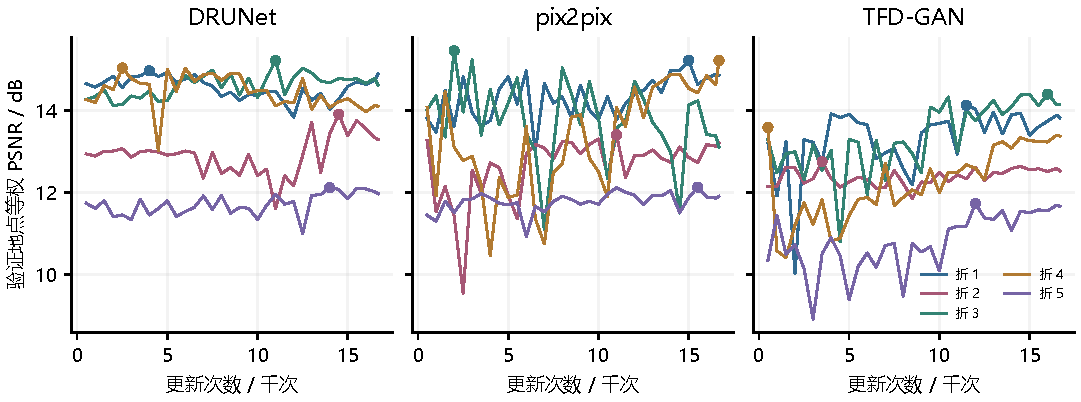
\includegraphics[width=\textwidth,height=.4\textheight,keepaspectratio]{figures/zh/results_20261109/validation_curves.pdf}
\caption{T124固定输入的五折验证轨迹（三模型五折共510个保存验证检查点）。\label{fig:s-training-monitor-zh}}
\end{figure}

\clearpage
\section*{补充节 4：全15对模态非SIFT几何审计明细与轨道C神经网络少样本微调}

\begin{table}[htbp]\centering\small
\caption{独立非SIFT梯度相位相关审计在全部15对模态上的汇总统计（432个有效$256\times256$图块，10倍亚像素上采样，$r_{\mathrm{grad}}\ge0.25$）。}\label{tab:s-geom-15pair-zh}
\begin{tabular}{@{}llrrrrr@{}}
\toprule
模态对 & 类别 & 可判定率/\% & 中位误差/px & RMSE/px & P95/px & $\le$2\,px占比/\%\\
\midrule
RGB--B1 & 跨模态 & 60.0 & 2.34 & 3.89 & 8.03 & 35.1\\
RGB--B2 & 跨模态 & 51.9 & 2.62 & 3.99 & 8.46 & 30.8\\
RGB--B3 & 跨模态 & 45.6 & 2.42 & 3.91 & 7.77 & 40.6\\
RGB--B4 & 跨模态 & 47.5 & 2.44 & 4.02 & 8.14 & 33.7\\
RGB--B5 & 跨模态 & 44.2 & 2.15 & 3.31 & 5.49 & 42.4\\
B1--B2 & SWIR波段间 & 90.7 & 0.28 & 1.46 & 2.07 & 94.4\\
B1--B3 & SWIR波段间 & 78.9 & 0.45 & 1.46 & 2.25 & 94.1\\
B1--B4 & SWIR波段间 & 85.2 & 0.45 & 1.70 & 3.44 & 91.3\\
B1--B5 & SWIR波段间 & 80.6 & 0.70 & 2.33 & 4.59 & 87.1\\
B2--B3 & SWIR波段间 & 79.2 & 0.51 & 1.90 & 2.91 & 90.4\\
B2--B4 & SWIR波段间 & 87.7 & 0.50 & 1.71 & 2.79 & 90.5\\
B2--B5 & SWIR波段间 & 79.4 & 0.72 & 2.02 & 3.19 & 88.3\\
B3--B4 & SWIR波段间 & 80.1 & 0.61 & 1.30 & 2.15 & 93.6\\
B3--B5 & SWIR波段间 & 78.2 & 0.63 & 1.58 & 2.82 & 91.1\\
B4--B5 & SWIR波段间 & 79.9 & 0.45 & 1.64 & 2.19 & 94.2\\
\midrule
\textbf{RGB--SWIR汇总（5对）} & -- & \textbf{49.8} & \textbf{2.37} & \textbf{3.85} & \textbf{7.97} & \textbf{36.2}\\
\textbf{SWIR--SWIR汇总（10对）} & -- & \textbf{82.0} & \textbf{0.51} & \textbf{1.73} & \textbf{2.84} & \textbf{91.5}\\
\bottomrule
\end{tabular}

\end{table}

\begin{figure}[htbp]\centering
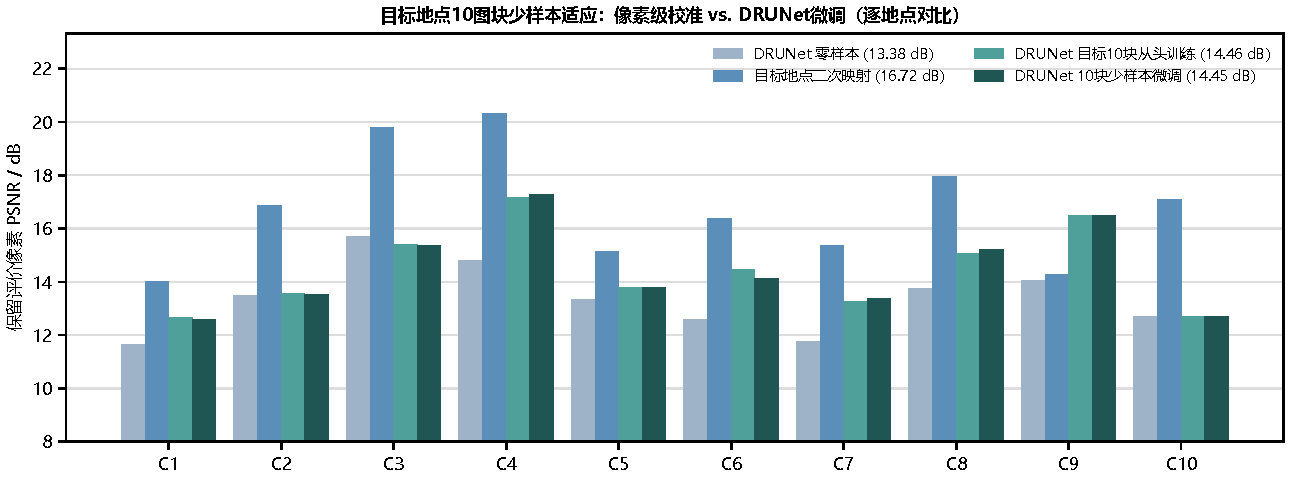
\includegraphics[width=\textwidth]{figures/zh/trackc_drunet_zh.pdf}
\caption{轨道C十个地点的目标10图块少样本适应逐地点对比（固定B1/B3/B4输入、同一50万保留像素）：DRUNet零样本、目标二次映射、DRUNet目标10块从头训练与DRUNet 10块少样本微调。\label{fig:s-trackc-drunet-zh}}
\end{figure}

\renewcommand{\bibfont}{\small}
\setlength{\bibsep}{2pt}
\bibliographystyle{unsrtnat}
\bibliography{refs}
\end{document}
